\documentclass[11pt, letterpaper]{article}

% Fonts and Encoding
\usepackage[utf8]{inputenc}
\usepackage[T1]{fontenc}
\usepackage{lmodern} % High-quality Latin Modern vector font

% Math and Symbols
\usepackage{amsmath, amssymb, amsthm, amsfonts, mathrsfs, mathtools}

% Layout and Geometry
\usepackage{geometry}
\geometry{letterpaper, margin=1in}
\setlength{\parindent}{0pt}
\setlength{\parskip}{0.6em}

% Formatting and Graphics
\usepackage{graphicx, xcolor, enumitem, booktabs, array, tabularx}

% TikZ for Illustrations
\usepackage{tikz}
\usetikzlibrary{arrows.meta, positioning, shapes.geometric, calc, backgrounds, matrix}

% Clickable Links and TOC
\usepackage{hyperref}
\hypersetup{
    colorlinks=true,
    linkcolor=blue,
    filecolor=magenta,      
    urlcolor=cyan,
    pdftitle={Advanced Mathematics Topic},
}

% Theorem Environments
\newtheorem{theorem}{Theorem}[section]
\newtheorem{lemma}[theorem]{Lemma}
\newtheorem{proposition}[theorem]{Proposition}
\newtheorem{corollary}[theorem]{Corollary}
\theoremstyle{definition}
\newtheorem{definition}{Definition}[section]
\newtheorem{axiom}{Axiom}[section]
\newtheorem{example}{Example}[section]
\theoremstyle{remark}
\newtheorem{remark}{Remark}[section]

% Custom Commands (Enforced standard notation)
\newcommand{\R}{\mathbb{R}}
\newcommand{\N}{\mathbb{N}}
\newcommand{\Z}{\mathbb{Z}}
\newcommand{\Q}{\mathbb{Q}}
\newcommand{\E}{\mathbb{E}}
\newcommand{\Prob}{\mathbb{P}}
\newcommand{\F}{\mathcal{F}}

\title{Section 7.2: Quadratic Forms --- Comprehensive Study Guide, Complete Solutions, and Theoretical Synthesis}
\author{Tashfeen Omran}
\date{\today}

\begin{document}

\maketitle
\tableofcontents
\newpage

% ============================================================================
% PART 1
% ============================================================================
\section{Part 1: Comprehensive Introduction, Context, and Prerequisites}

\subsection{Core Concepts of Quadratic Forms}

Up to this stage in linear algebra, primary attention is devoted to linear equations and linear transformations of the form $\mathbf{x} \mapsto A\mathbf{x}$, alongside inner products $\mathbf{x}^T \mathbf{x} = \|\mathbf{x}\|^2$. In science, engineering, geometry, and statistics, however, one constantly encounters homogeneous second-degree polynomials in several variables. These expressions are known as \textbf{quadratic forms}.

\begin{definition}[Quadratic Form and Matrix of a Quadratic Form]
A \textbf{quadratic form} on $\R^n$ is a real-valued function $Q : \R^n \to \R$ whose value at any vector $\mathbf{x} = (x_1, x_2, \dots, x_n)^T \in \R^n$ can be computed by an expression of the form
\[
Q(\mathbf{x}) = \mathbf{x}^T A \mathbf{x},
\]
where $A = [a_{ij}]$ is an $n \times n$ \textbf{symmetric matrix} ($A^T = A$). The symmetric matrix $A$ is called the \textbf{matrix of the quadratic form}.
\end{definition}

Expanding the matrix product $\mathbf{x}^T A \mathbf{x}$ for a symmetric $n \times n$ matrix $A$ reveals the exact algebraic anatomy of any quadratic form:
\[
Q(\mathbf{x}) = \sum_{i=1}^{n} \sum_{j=1}^{n} a_{ij} x_i x_j = \sum_{i=1}^{n} a_{ii} x_i^2 + 2 \sum_{1 \le i < j \le n} a_{ij} x_i x_j.
\]
Two distinct types of terms appear in this polynomial expansion:
\begin{itemize}
    \item \textbf{Squared (Diagonal) Terms} ($a_{ii} x_i^2$): Controlled exclusively by the main diagonal entries $a_{11}, a_{22}, \dots, a_{nn}$ of $A$.
    \item \textbf{Cross-Product Terms} ($2 a_{ij} x_i x_j$ for $i < j$): Controlled by the off-diagonal entries of $A$. Because $A$ is symmetric ($a_{ij} = a_{ji}$), the total coefficient $c_{ij}$ multiplying $x_i x_j$ ($i \neq j$) in the polynomial is split evenly between the $(i,j)$-entry and the $(j,i)$-entry: $a_{ij} = a_{ji} = \frac{1}{2} c_{ij}$.
\end{itemize}
The simplest nonzero quadratic form on $\R^n$ is $Q(\mathbf{x}) = \mathbf{x}^T I_n \mathbf{x} = x_1^2 + x_2^2 + \dots + x_n^2 = \|\mathbf{x}\|^2$, whose symmetric matrix is the identity matrix $I_n$. More generally, whenever $A = D = \operatorname{diag}(d_1, \dots, d_n)$ is a diagonal matrix, $Q(\mathbf{x}) = d_1 x_1^2 + \dots + d_n x_n^2$ has \emph{no cross-product terms}.

When cross-product terms are present, analyzing the geometry or sign behavior of $Q(\mathbf{x})$ directly in the standard coordinates $(x_1, \dots, x_n)$ is difficult because variables interact. To decouple them, we introduce a \textbf{change of variable}:
\[
\mathbf{x} = P\mathbf{y}, \quad \text{or equivalently,} \quad \mathbf{y} = P^{-1}\mathbf{x},
\]
where $P$ is an invertible $n \times n$ matrix and $\mathbf{y} \in \R^n$ is the coordinate vector of $\mathbf{x}$ relative to the basis formed by the columns of $P$. If $P$ is chosen to be an \textbf{orthogonal matrix} ($P^{-1} = P^T$) that orthogonally diagonalizes $A$, the cross-product terms vanish completely, and the columns of $P$ define the \textbf{principal axes} of the quadratic form.

Finally, because $Q(\mathbf{x}) = \mathbf{x}^T A \mathbf{x}$ is a scalar-valued function on $\R^n$ satisfying $Q(\mathbf{0}) = 0$, we classify quadratic forms (and correspondingly their symmetric matrices $A$) according to the signs of the values $Q(\mathbf{x})$ for $\mathbf{x} \neq \mathbf{0}$:

\begin{definition}[Definiteness Classification of Quadratic Forms]
Let $Q : \R^n \to \R$ be a quadratic form $Q(\mathbf{x}) = \mathbf{x}^T A \mathbf{x}$. Then $Q$ (and the symmetric matrix $A$) is said to be:
\begin{enumerate}[label=\alph*.]
    \item \textbf{Positive definite} if $Q(\mathbf{x}) > 0$ for all $\mathbf{x} \neq \mathbf{0}$.
    \item \textbf{Negative definite} if $Q(\mathbf{x}) < 0$ for all $\mathbf{x} \neq \mathbf{0}$.
    \item \textbf{Indefinite} if $Q(\mathbf{x})$ assumes both strictly positive and strictly negative values.
    \item \textbf{Positive semidefinite} if $Q(\mathbf{x}) \ge 0$ for all $\mathbf{x} \in \R^n$.
    \item \textbf{Negative semidefinite} if $Q(\mathbf{x}) \le 0$ for all $\mathbf{x} \in \R^n$.
\end{enumerate}
\end{definition}

\subsection{Intuition and Mathematical Derivation}

\textbf{1. Why Require $A$ to Be Symmetric?}
Suppose we start with an arbitrary (possibly non-symmetric) $n \times n$ matrix $B$ and form the scalar expression $\mathbf{x}^T B \mathbf{x}$. Since $\mathbf{x}^T B \mathbf{x}$ is a $1 \times 1$ matrix (a scalar), it equals its own transpose:
\[
\mathbf{x}^T B \mathbf{x} = (\mathbf{x}^T B \mathbf{x})^T = \mathbf{x}^T B^T (\mathbf{x}^T)^T = \mathbf{x}^T B^T \mathbf{x}.
\]
Averaging these two identical expressions gives
\[
\mathbf{x}^T B \mathbf{x} = \frac{1}{2}\left(\mathbf{x}^T B \mathbf{x} + \mathbf{x}^T B^T \mathbf{x}\right) = \mathbf{x}^T \left(\frac{B + B^T}{2}\right) \mathbf{x}.
\]
Setting $A = \frac{1}{2}(B + B^T)$, we observe that $A^T = A$. Without restricting $A$ to be symmetric, infinitely many matrices would represent the exact same quadratic polynomial (for instance, $\begin{bmatrix} 3 & -4 \\ 0 & 7 \end{bmatrix}$ and $\begin{bmatrix} 3 & -2 \\ -2 & 7 \end{bmatrix}$ both yield $3x_1^2 - 4x_1x_2 + 7x_2^2$). Enforcing symmetry guarantees a \emph{unique, one-to-one correspondence} between quadratic forms on $\R^n$ and $n \times n$ real symmetric matrices, while simultaneously unlocking the Spectral Theorem for symmetric matrices.

\textbf{2. Derivation of the Principal Axes Theorem.}
Substitute the linear change of variable $\mathbf{x} = P\mathbf{y}$ into $Q(\mathbf{x}) = \mathbf{x}^T A \mathbf{x}$ and apply the transpose reversal law $(P\mathbf{y})^T = \mathbf{y}^T P^T$:
\[
\mathbf{x}^T A \mathbf{x} = (P\mathbf{y})^T A (P\mathbf{y}) = \mathbf{y}^T P^T A P \mathbf{y} = \mathbf{y}^T (P^T A P) \mathbf{y}.
\]
Notice that $(P^T A P)^T = P^T A^T (P^T)^T = P^T A P$, so the new matrix of the quadratic form in $\mathbf{y}$-coordinates is $P^T A P$. Because $A$ is real and symmetric, the Spectral Theorem (Section 7.1, Theorem 2) guarantees that $A$ is orthogonally diagonalizable: there exists an orthogonal matrix $P = \begin{bmatrix} \mathbf{u}_1 & \mathbf{u}_2 & \dots & \mathbf{u}_n \end{bmatrix}$ whose columns are orthonormal eigenvectors of $A$ ($P^{-1} = P^T$) such that
\[
P^T A P = P^{-1} A P = D = \begin{bmatrix} \lambda_1 & 0 & \cdots & 0 \\ 0 & \lambda_2 & \cdots & 0 \\ \vdots & \vdots & \ddots & \vdots \\ 0 & 0 & \cdots & \lambda_n \end{bmatrix}.
\]
Consequently, under $\mathbf{x} = P\mathbf{y}$, the quadratic form collapses into a pure weighted sum of squares:
\[
Q(\mathbf{x}) = \mathbf{y}^T D \mathbf{y} = \lambda_1 y_1^2 + \lambda_2 y_2^2 + \dots + \lambda_n y_n^2.
\]

\begin{theorem}[Theorem 4: The Principal Axes Theorem]
Let $A$ be an $n \times n$ symmetric matrix. Then there is an orthogonal change of variable, $\mathbf{x} = P\mathbf{y}$, that transforms the quadratic form $\mathbf{x}^T A \mathbf{x}$ into a quadratic form $\mathbf{y}^T D \mathbf{y}$ with no cross-product term.
\end{theorem}

\textbf{3. Geometric Intuition of Principal Axes.}
In $\R^2$, when $A$ is invertible and $c \neq 0$ is a constant, the level curve $\mathbf{x}^T A \mathbf{x} = c$ represents an ellipse (or circle), a hyperbola, or the empty set (and when $c = 0$ or $\det A = 0$, intersecting lines, parallel lines, or a single point). Cross-product terms $2a_{12}x_1x_2$ tilt the conic section out of standard alignment with the $x_1$- and $x_2$-axes. Because $P$ is orthogonal ($P^T P = I$), multiplication by $P$ preserves all lengths and angles ($\|P\mathbf{y}\| = \|\mathbf{y}\|$): it represents a rigid rotation (possibly composed with a reflection). Choosing $\det P = +1$ rotates the coordinate axes to align precisely with the symmetry axes (principal axes) $\mathbf{u}_1, \mathbf{u}_2$ of the conic, placing the equation into unrotated standard position $\lambda_1 y_1^2 + \lambda_2 y_2^2 = c$.

\begin{center}
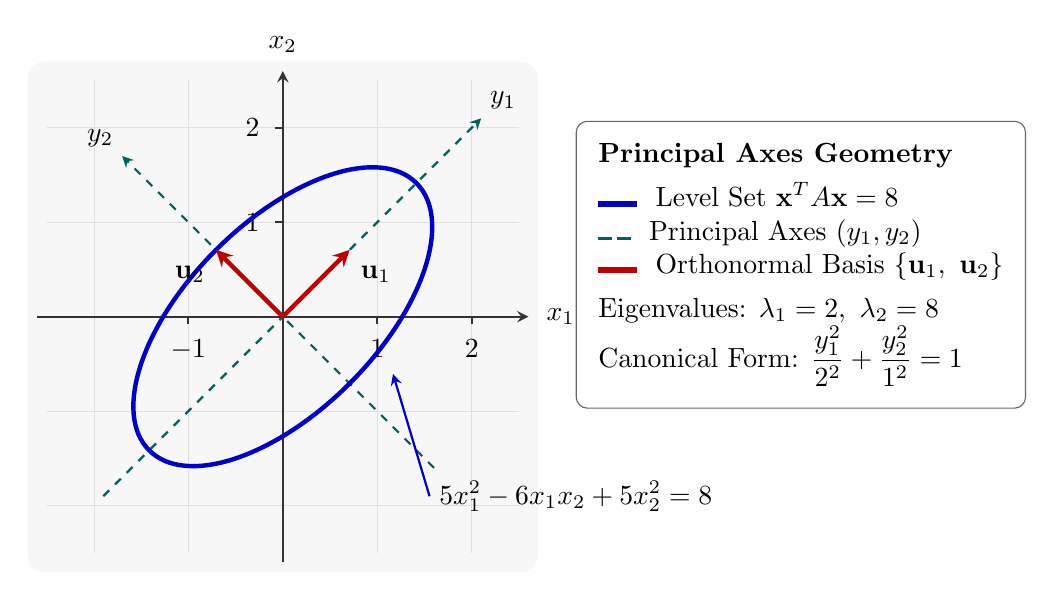
\begin{tikzpicture}[scale=1.2]
    % 1) Background Layer
    \fill[gray!6, rounded corners=6pt] (-2.7,-2.7) rectangle (2.7,2.7);

    % 2) Grid Lines and Coordinate Axes
    \draw[step=1.0, gray!25, very thin] (-2.5,-2.5) grid (2.5,2.5);
    \draw[->, >=stealth, thick, black!80] (-2.6,0) -- (2.6,0);
    \draw[->, >=stealth, thick, black!80] (0,-2.6) -- (0,2.6);

    % Microscopic tick marks on standard axes
    \draw[thick, black!80] (1,0) -- (1,-0.08) node[below=2pt, text=black] {$1$};
    \draw[thick, black!80] (2,0) -- (2,-0.08) node[below=2pt, text=black] {$2$};
    \draw[thick, black!80] (-1,0) -- (-1,-0.08) node[below=2pt, text=black] {$-1$};
    \draw[thick, black!80] (0,1) -- (-0.08,1) node[left=2pt, text=black] {$1$};
    \draw[thick, black!80] (0,2) -- (-0.08,2) node[left=2pt, text=black] {$2$};

    % Rotated Principal Axes (y_1, y_2)
    \draw[->, >=stealth, thick, dashed, teal!75!black] (-1.9,-1.9) -- (2.1,2.1);
    \draw[->, >=stealth, thick, dashed, teal!75!black] (1.6,-1.6) -- (-1.7,1.7);

    % 3) Primary Plot: Rotated Ellipse 5x_1^2 - 6x_1x_2 + 5x_2^2 = 8  <=>  2y_1^2 + 8y_2^2 = 8
    \draw[rotate=45, ultra thick, blue!80!black] (0,0) ellipse (2 and 1);

    % Unit Eigenvectors (Principal Axes Basis Vectors)
    \draw[->, >=stealth, ultra thick, red!75!black] (0,0) -- (0.7071,0.7071);
    \draw[->, >=stealth, ultra thick, red!75!black] (0,0) -- (-0.7071,0.7071);

    % 4) Labels, Off-Axis Callouts, and Single-Node Multiline Legend
    \node[right=3pt, text=black] at (2.6,0) {$x_1$};
    \node[above=3pt, text=black] at (0,2.6) {$x_2$};
    \node[above right=2pt, text=black] at (2.05,2.05) {$y_1$};
    \node[above left=2pt, text=black] at (-1.65,1.65) {$y_2$};

    \node[below right=2pt, text=black] at (0.68,0.68) {$\mathbf{u}_1$};
    \node[below left=2pt, text=black] at (-0.68,0.68) {$\mathbf{u}_2$};

    % Off-axis callout pointing to rotated ellipse
    \node[text=black, align=left] (callout) at (3.1,-1.9) {$\displaystyle 5x_1^2 - 6x_1x_2 + 5x_2^2 = 8$};
    \draw[->, >=stealth, shorten >=2pt, thick, blue!80!black] (callout.west) -- (1.15,-0.55);

    % Single-Node Multiline Legend anchored West in open right margin
    \node[draw=black!60, fill=white, rounded corners=4pt, inner sep=8pt, align=left, anchor=west, text=black] at (3.1,0.55) {
        \textbf{Principal Axes Geometry}\\[4pt]
        \textcolor{blue!80!black}{\rule{14pt}{2.2pt}}\ \ Level Set $\displaystyle \mathbf{x}^T A \mathbf{x} = 8$\\
        \textcolor{teal!75!black}{\rule{5pt}{1.2pt}\,\rule{5pt}{1.2pt}}\ \ Principal Axes $(y_1, y_2)$\\
        \textcolor{red!75!black}{\rule{14pt}{2.2pt}}\ \ Orthonormal Basis $\{\mathbf{u}_1,\ \mathbf{u}_2\}$\\[4pt]
        Eigenvalues: $\displaystyle \lambda_1 = 2,\ \lambda_2 = 8$\\
        Canonical Form: $\displaystyle \frac{y_1^2}{2^2} + \frac{y_2^2}{1^2} = 1^{\vphantom{A}}$
    };
\end{tikzpicture}
\end{center}

\textbf{4. Derivation of Eigenvalue Classification (Theorem 5).}
Because $P$ in $\mathbf{x} = P\mathbf{y}$ is invertible, $\mathbf{x} \neq \mathbf{0}$ if and only if $\mathbf{y} \neq \mathbf{0}$. Thus the range of values assumed by $Q(\mathbf{x})$ for $\mathbf{x} \neq \mathbf{0}$ is identical to the range of values assumed by
\[
\mathbf{y}^T D \mathbf{y} = \lambda_1 y_1^2 + \lambda_2 y_2^2 + \dots + \lambda_n y_n^2 \quad \text{for } \mathbf{y} \neq \mathbf{0}.
\]
\begin{itemize}
    \item If every $\lambda_i > 0$, then for any $\mathbf{y} \neq \mathbf{0}$ at least one $y_k \neq 0$, so $\lambda_k y_k^2 > 0$ and all other terms $\lambda_i y_i^2 \ge 0$; hence $Q(\mathbf{x}) > 0$. Conversely, if $Q(\mathbf{x}) > 0$ for all $\mathbf{x} \neq \mathbf{0}$, evaluating at $\mathbf{x} = P\mathbf{e}_i \neq \mathbf{0}$ (so $\mathbf{y} = \mathbf{e}_i$) gives $Q(P\mathbf{e}_i) = \lambda_i (1)^2 = \lambda_i > 0$ for each $i$.
    \item Symmetrically, $Q(\mathbf{x}) < 0$ for all $\mathbf{x} \neq \mathbf{0}$ if and only if $\lambda_i < 0$ for all $i$.
    \item If $\lambda_j > 0$ and $\lambda_k < 0$ for some indices $j, k$, then $Q(P\mathbf{e}_j) = \lambda_j > 0$ and $Q(P\mathbf{e}_k) = \lambda_k < 0$, so $Q$ is indefinite. Conversely, if $Q$ takes both positive and negative values, its eigenvalues cannot all be $\ge 0$ (which would force $Q \ge 0$) nor all $\le 0$ (which would force $Q \le 0$), so $A$ must have at least one strictly positive and at least one strictly negative eigenvalue.
\end{itemize}

\begin{theorem}[Theorem 5: Quadratic Forms and Eigenvalues]
Let $A$ be an $n \times n$ symmetric matrix. Then a quadratic form $\mathbf{x}^T A \mathbf{x}$ is:
\begin{enumerate}[label=\alph*.]
    \item \textbf{positive definite} if and only if the eigenvalues of $A$ are all positive,
    \item \textbf{negative definite} if and only if the eigenvalues of $A$ are all negative, or
    \item \textbf{indefinite} if and only if $A$ has both positive and negative eigenvalues.
\end{enumerate}
\end{theorem}

\subsection{Historical Context and Scientific Motivation}

The theory of quadratic forms emerged at the crossroads of number theory, analytical mechanics, and celestial geometry during the eighteenth and nineteenth centuries. In pure mathematics, Pierre de Fermat, Leonhard Euler, Joseph-Louis Lagrange, and Carl Friedrich Gauss (in his monumental 1801 treatise \emph{Disquisitiones Arithmeticae}) studied binary and ternary integer quadratic forms $ax^2 + 2bxy + cy^2$ to answer deep arithmetic questions about which integers can be represented as sums of squares, introducing equivalence transformations $\mathbf{x} = P\mathbf{y}$ and the discriminant $b^2 - ac$. Concurrently, in his 1788 \emph{M\'{e}canique Analytique}, Lagrange modeled small mechanical oscillations of coupled pendulums and planetary orbits near equilibrium: both the kinetic energy $T(\dot{\mathbf{q}}) = \frac{1}{2}\dot{\mathbf{q}}^T M \dot{\mathbf{q}}$ and the local potential energy $V(\mathbf{q}) \approx \frac{1}{2}\mathbf{q}^T K \mathbf{q}$ are quadratic forms, and physical stability of equilibrium required $V(\mathbf{q}) > 0$ for every nonzero displacement $\mathbf{q} \neq \mathbf{0}$---the exact physical birth of positive definiteness.

In 1829, Augustin-Louis Cauchy resolved a major problem in celestial mechanics and rigid-body dynamics: finding the principal axes of inertia of a three-dimensional body and classifying quadric surfaces $\mathbf{x}^T A \mathbf{x} = c$ in $\R^3$. In his celebrated memoir \emph{Sur l'\'{e}quation \`{a} l'aide de laquelle on d\'{e}termine les in\'{e}galit\'{e}s s\'{e}culaires des mouvements des plan\`{e}tes}, Cauchy proved for the first time that every real symmetric matrix possesses exclusively real roots (eigenvalues) and orthogonal principal axes, establishing the Principal Axes Theorem. Two decades later, James Joseph Sylvester (1851--1852) coined the modern matrix terminology, proved the Law of Inertia (showing that the counts of positive, negative, and zero coefficients in any diagonalized form are invariant), and established determinantal tests for definiteness, laying the algebraic foundation for modern optimization, Riemannian geometry, quantum mechanics, and multivariate statistics.

\subsection{Essential Formulas and Theorems Summary}

\renewcommand{\arraystretch}{1.5}
\begin{tabularx}{\textwidth}{l >{$\displaystyle}l<{$} X}
\toprule
\textbf{Concept} & \multicolumn{1}{l}{\textbf{Canonical Formula}} & \textbf{Interpretation and Conditions} \\
\midrule
Quadratic Form & Q(\mathbf{x}) = \mathbf{x}^T A \mathbf{x} & $A = A^T$ is the unique $n \times n$ symmetric matrix of $Q$. \\
Matrix Entries & a_{ii} = c_{ii},\ \ a_{ij} = a_{ji} = \frac{1}{2}c_{ij} & $c_{ii}$ is coefficient of $x_i^2$; $c_{ij}$ ($i \neq j$) is coefficient of $x_i x_j$. \\
Change of Variable & \mathbf{x} = P\mathbf{y} \iff \mathbf{y} = P^{-1}\mathbf{x} & Transforms $\mathbf{x}^T A \mathbf{x}$ into $\mathbf{y}^T (P^T A P) \mathbf{y}$. \\
Principal Axes Form & \mathbf{x}^T A \mathbf{x} = \mathbf{y}^T D \mathbf{y} = \sum_{i=1}^n \lambda_i y_i^2^{\vphantom{A}} & $P$ orthogonal ($P^T = P^{-1}$), columns $\mathbf{u}_i$ are unit eigenvectors of $A$, $D = \operatorname{diag}(\lambda_1, \dots, \lambda_n)$. \\
\addlinespace[4pt]
Positive Definite & Q(\mathbf{x}) > 0\ (\forall \mathbf{x} \neq \mathbf{0}) \iff \lambda_i > 0\ (\forall i) & Upward elliptic paraboloid; level sets $\mathbf{x}^T A \mathbf{x} = c > 0$ are ellipsoids. \\
Negative Definite & Q(\mathbf{x}) < 0\ (\forall \mathbf{x} \neq \mathbf{0}) \iff \lambda_i < 0\ (\forall i) & Downward elliptic paraboloid; $-A$ is positive definite. \\
Indefinite & \exists\, \mathbf{u}, \mathbf{v} : Q(\mathbf{u}) > 0 > Q(\mathbf{v}) \iff \exists\, \lambda_j > 0 > \lambda_k & Hyperbolic saddle surface; level sets in $\R^2$ are hyperbolas or lines. \\
Positive Semidefinite & Q(\mathbf{x}) \ge 0\ (\forall \mathbf{x}) \iff \lambda_i \ge 0\ (\forall i) & Includes positive definite forms plus degenerate troughs with $\lambda_i = 0$. \\
Negative Semidefinite & Q(\mathbf{x}) \le 0\ (\forall \mathbf{x}) \iff \lambda_i \le 0\ (\forall i) & Includes negative definite forms plus degenerate ridges with $\lambda_i = 0$. \\
Cholesky Factorization & A = R^T R & Exists with $R$ upper triangular with positive diagonal entries iff $A$ is positive definite. \\
\bottomrule
\end{tabularx}

\subsection{Essential Prerequisites}

To master Section 7.2 without friction, you must have command of the following foundational tools:
\begin{enumerate}
    \item \textbf{Matrix Multiplication and Transpose Laws}: Computing row-by-matrix-by-column products $\mathbf{x}^T A \mathbf{x}$ and applying $(AB)^T = B^T A^T$ and $(A^{-1})^T = (A^T)^{-1}$.
    \item \textbf{Coordinate Vectors Relative to a Basis (Section 4.4)}: Understanding that $\mathbf{x} = P\mathbf{y}$ expresses $\mathbf{x}$ as $y_1 \mathbf{p}_1 + \dots + y_n \mathbf{p}_n$, so $\mathbf{y} = [\mathbf{x}]_{\mathcal{B}} = P^{-1}\mathbf{x}$ gives coordinates in the new basis $\mathcal{B} = \{\mathbf{p}_1, \dots, \mathbf{p}_n\}$.
    \item \textbf{Eigenvalues and Eigenspaces (Chapter 5)}: Computing the characteristic polynomial $\det(A - \lambda I) = 0$, factoring polynomials, and row-reducing $(A - \lambda I)\mathbf{x} = \mathbf{0}$ to parametric vector form to find eigenspace bases.
    \item \textbf{Inner Products, Norms, and the Gram--Schmidt Process (Chapter 6)}: Computing $\mathbf{u} \cdot \mathbf{v} = \mathbf{u}^T \mathbf{v}$, normalizing $\mathbf{u} = \mathbf{v}/\|\mathbf{v}\|$, and orthogonalizing a basis $\{\mathbf{w}_1, \mathbf{w}_2\}$ via $\mathbf{v}_2 = \mathbf{w}_2 - \frac{\mathbf{w}_2 \cdot \mathbf{v}_1}{\mathbf{v}_1 \cdot \mathbf{v}_1}\mathbf{v}_1$.
    \item \textbf{Orthogonal Diagonalization of Symmetric Matrices (Section 7.1)}: Knowing that eigenvectors from distinct eigenspaces of a symmetric matrix $A$ are automatically orthogonal, while eigenspaces of dimension $\ge 2$ require Gram--Schmidt to construct an orthogonal matrix $P$ ($P^T P = I$) satisfying $A = P D P^T$.
\end{enumerate}

\newpage
% ============================================================================
% PART 2
% ============================================================================
\section{Part 2: Detailed Homework Solutions}

\subsection{Practice Problem}

\textbf{Original Problem.} Describe a positive semidefinite matrix $A$ in terms of its eigenvalues.

\textbf{Solution.}
Let $A$ be an $n \times n$ symmetric matrix. By definition, $A$ is positive semidefinite if and only if its quadratic form satisfies $\mathbf{x}^T A \mathbf{x} \ge 0$ for all $\mathbf{x} \in \R^n$. By the Principal Axes Theorem (Theorem 4), there exists an orthogonal matrix $P$ ($P^{-1} = P^T$) such that the change of variable $\mathbf{x} = P\mathbf{y}$ transforms $\mathbf{x}^T A \mathbf{x}$ into
\[
\mathbf{x}^T A \mathbf{x} = \mathbf{y}^T D \mathbf{y} = \lambda_1 y_1^2 + \lambda_2 y_2^2 + \dots + \lambda_n y_n^2,
\]
where $\lambda_1, \lambda_2, \dots, \lambda_n$ are the eigenvalues of $A$.

\begin{itemize}
    \item $(\implies)$ Suppose $A$ is positive semidefinite, so $\mathbf{x}^T A \mathbf{x} \ge 0$ for all $\mathbf{x} \in \R^n$. Assume for contradiction that some eigenvalue $\lambda_i < 0$. Choose $\mathbf{y} = \mathbf{e}_i$ (the $i$-th column of $I_n$, having $1$ in entry $i$ and $0$ elsewhere) and let $\mathbf{x} = P\mathbf{e}_i$. Then
    \[
    \mathbf{x}^T A \mathbf{x} = \mathbf{e}_i^T D \mathbf{e}_i = \lambda_i (1)^2 = \lambda_i < 0,
    \]
    which contradicts $\mathbf{x}^T A \mathbf{x} \ge 0$. Hence every eigenvalue satisfies $\lambda_i \ge 0$.
    \item $(\Longleftarrow)$ Conversely, suppose $\lambda_i \ge 0$ for all $i = 1, \dots, n$. Since $y_i^2 \ge 0$ for every real number $y_i$, each product $\lambda_i y_i^2 \ge 0$. Summing over $i = 1, \dots, n$ yields
    \[
    \mathbf{x}^T A \mathbf{x} = \lambda_1 y_1^2 + \lambda_2 y_2^2 + \dots + \lambda_n y_n^2 \ge 0 \quad \text{for all } \mathbf{x} \in \R^n.
    \]
    Hence $A$ is positive semidefinite.
\end{itemize}

\textbf{Final Answer:} A symmetric matrix $A$ is positive semidefinite if and only if all of its eigenvalues are nonnegative ($\lambda_i \ge 0$ for all $i$).

\subsection{Exercises 1--6: Computing Quadratic Forms and Finding Symmetric Matrices}

\textbf{Exercise 1 --- Original Problem.} Compute the quadratic form $\mathbf{x}^T A \mathbf{x}$, when $A = \begin{bmatrix} 3 & 1/4 \\ 1/4 & 1 \end{bmatrix}$ and:
\begin{enumerate}[label=\alph*.]
    \item $\mathbf{x} = \begin{bmatrix} x_1 \\ x_2 \end{bmatrix}$
    \item $\mathbf{x} = \begin{bmatrix} 8 \\ 1 \end{bmatrix}$
    \item $\mathbf{x} = \begin{bmatrix} 1 \\ 4 \end{bmatrix}$
\end{enumerate}

\textbf{Solution.}
\begin{enumerate}[label=\alph*.]
    \item First compute $A\mathbf{x}$, then left-multiply by $\mathbf{x}^T$:
    \begin{align*}
    \mathbf{x}^T A \mathbf{x} &= \begin{bmatrix} x_1 & x_2 \end{bmatrix} \begin{bmatrix} 3 & 1/4 \\ 1/4 & 1 \end{bmatrix} \begin{bmatrix} x_1 \\ x_2 \end{bmatrix} = \begin{bmatrix} x_1 & x_2 \end{bmatrix} \begin{bmatrix} 3x_1 + \frac{1}{4}x_2 \\[4pt] \frac{1}{4}x_1 + x_2 \end{bmatrix} \\
    &= x_1\left(3x_1 + \frac{1}{4}x_2\right) + x_2\left(\frac{1}{4}x_1 + x_2\right) \\
    &= 3x_1^2 + \frac{1}{4}x_1x_2 + \frac{1}{4}x_2x_1 + x_2^2 = 3x_1^2 + \frac{1}{2}x_1x_2 + x_2^2.
    \end{align*}
    \item For $\mathbf{x} = \begin{bmatrix} 8 \\ 1 \end{bmatrix}$:
    \[
    \mathbf{x}^T A \mathbf{x} = \begin{bmatrix} 8 & 1 \end{bmatrix} \begin{bmatrix} 3 & 1/4 \\ 1/4 & 1 \end{bmatrix} \begin{bmatrix} 8 \\ 1 \end{bmatrix} = \begin{bmatrix} 8 & 1 \end{bmatrix} \begin{bmatrix} 24 + \frac{1}{4} \\[4pt] 2 + 1 \end{bmatrix} = \begin{bmatrix} 8 & 1 \end{bmatrix} \begin{bmatrix} 97/4 \\ 3 \end{bmatrix} = 8\left(\frac{97}{4}\right) + 1(3) = 194 + 3 = 197.
    \]
    (Check via part (a): $3(8)^2 + \frac{1}{2}(8)(1) + (1)^2 = 192 + 4 + 1 = 197$.)
    \item For $\mathbf{x} = \begin{bmatrix} 1 \\ 4 \end{bmatrix}$:
    \[
    \mathbf{x}^T A \mathbf{x} = \begin{bmatrix} 1 & 4 \end{bmatrix} \begin{bmatrix} 3 & 1/4 \\ 1/4 & 1 \end{bmatrix} \begin{bmatrix} 1 \\ 4 \end{bmatrix} = \begin{bmatrix} 1 & 4 \end{bmatrix} \begin{bmatrix} 3 + 1 \\[4pt] \frac{1}{4} + 4 \end{bmatrix} = \begin{bmatrix} 1 & 4 \end{bmatrix} \begin{bmatrix} 4 \\ 17/4 \end{bmatrix} = 1(4) + 4\left(\frac{17}{4}\right) = 4 + 17 = 21.
    \]
    (Check via part (a): $3(1)^2 + \frac{1}{2}(1)(4) + (4)^2 = 3 + 2 + 16 = 21$.)
\end{enumerate}

\textbf{Final Answer:} (a) $3x_1^2 + \frac{1}{2}x_1x_2 + x_2^2$; \quad (b) $197$; \quad (c) $21$.

\medskip
\hrule
\medskip

\textbf{Exercise 2 --- Original Problem.} Compute the quadratic form $\mathbf{x}^T A \mathbf{x}$, for $A = \begin{bmatrix} 4 & 1 & 0 \\ 1 & 1 & 3 \\ 0 & 3 & 0 \end{bmatrix}$ and:
\begin{enumerate}[label=\alph*.]
    \item $\mathbf{x} = \begin{bmatrix} x_1 \\ x_2 \\ x_3 \end{bmatrix}$
    \item $\mathbf{x} = \begin{bmatrix} -3 \\ -1 \\ 4 \end{bmatrix}$
    \item $\mathbf{x} = \begin{bmatrix} 1/\sqrt{5} \\ 1/\sqrt{5} \\ 1/\sqrt{5} \end{bmatrix}$
\end{enumerate}

\textbf{Solution.}
\begin{enumerate}[label=\alph*.]
    \item Compute $A\mathbf{x}$ and multiply on the left by $\mathbf{x}^T$:
    \begin{align*}
    \mathbf{x}^T A \mathbf{x} &= \begin{bmatrix} x_1 & x_2 & x_3 \end{bmatrix} \begin{bmatrix} 4 & 1 & 0 \\ 1 & 1 & 3 \\ 0 & 3 & 0 \end{bmatrix} \begin{bmatrix} x_1 \\ x_2 \\ x_3 \end{bmatrix} = \begin{bmatrix} x_1 & x_2 & x_3 \end{bmatrix} \begin{bmatrix} 4x_1 + x_2 \\ x_1 + x_2 + 3x_3 \\ 3x_2 \end{bmatrix} \\
    &= x_1(4x_1 + x_2) + x_2(x_1 + x_2 + 3x_3) + x_3(3x_2) \\
    &= 4x_1^2 + x_1x_2 + x_2x_1 + x_2^2 + 3x_2x_3 + 3x_3x_2 \\
    &= 4x_1^2 + x_2^2 + 2x_1x_2 + 6x_2x_3.
    \end{align*}
    \item For $\mathbf{x} = \begin{bmatrix} -3 \\ -1 \\ 4 \end{bmatrix}$:
    \begin{align*}
    \mathbf{x}^T A \mathbf{x} &= \begin{bmatrix} -3 & -1 & 4 \end{bmatrix} \begin{bmatrix} 4 & 1 & 0 \\ 1 & 1 & 3 \\ 0 & 3 & 0 \end{bmatrix} \begin{bmatrix} -3 \\ -1 \\ 4 \end{bmatrix} = \begin{bmatrix} -3 & -1 & 4 \end{bmatrix} \begin{bmatrix} -12 - 1 + 0 \\ -3 - 1 + 12 \\ 0 - 3 + 0 \end{bmatrix} \\
    &= \begin{bmatrix} -3 & -1 & 4 \end{bmatrix} \begin{bmatrix} -13 \\ 8 \\ -3 \end{bmatrix} = (-3)(-13) + (-1)(8) + (4)(-3) = 39 - 8 - 12 = 19.
    \end{align*}
    (Check via part (a): $4(-3)^2 + (-1)^2 + 2(-3)(-1) + 6(-1)(4) = 36 + 1 + 6 - 24 = 19$.)
    \item Factor out $\frac{1}{\sqrt{5}}$ from $\mathbf{x} = \frac{1}{\sqrt{5}} \begin{bmatrix} 1 \\ 1 \\ 1 \end{bmatrix}$:
    \begin{align*}
    \mathbf{x}^T A \mathbf{x} &= \left(\frac{1}{\sqrt{5}}\right)^2 \begin{bmatrix} 1 & 1 & 1 \end{bmatrix} \begin{bmatrix} 4 & 1 & 0 \\ 1 & 1 & 3 \\ 0 & 3 & 0 \end{bmatrix} \begin{bmatrix} 1 \\ 1 \\ 1 \end{bmatrix} = \frac{1}{5} \begin{bmatrix} 1 & 1 & 1 \end{bmatrix} \begin{bmatrix} 5 \\ 5 \\ 3 \end{bmatrix} = \frac{1}{5}(5 + 5 + 3) = \frac{13}{5}.
    \end{align*}
\end{enumerate}

\textbf{Final Answer:} (a) $4x_1^2 + x_2^2 + 2x_1x_2 + 6x_2x_3$; \quad (b) $19$; \quad (c) $\frac{13}{5}$.

\medskip
\hrule
\medskip

\textbf{Exercise 3 --- Original Problem.} Find the matrix of the quadratic form. Assume $\mathbf{x}$ is in $\R^2$.
\begin{enumerate}[label=\alph*.]
    \item $4x_1^2 - 6x_1x_2 + 5x_2^2$
    \item $5x_1^2 + 4x_1x_2$
\end{enumerate}

\textbf{Solution.}
Place the coefficients of $x_1^2$ and $x_2^2$ on the main diagonal $(a_{11}, a_{22})$, and split the coefficient of $x_1x_2$ evenly between $a_{12}$ and $a_{21}$:
\begin{enumerate}[label=\alph*.]
    \item Here $a_{11} = 4$, $a_{22} = 5$, and $a_{12} = a_{21} = \frac{-6}{2} = -3$. Thus $A = \begin{bmatrix} 4 & -3 \\ -3 & 5 \end{bmatrix}$.
    \item Since there is no $x_2^2$ term, its coefficient is $0$. Thus $a_{11} = 5$, $a_{22} = 0$, and $a_{12} = a_{21} = \frac{4}{2} = 2$, giving $A = \begin{bmatrix} 5 & 2 \\ 2 & 0 \end{bmatrix}$.
\end{enumerate}

\textbf{Final Answer:} (a) $\begin{bmatrix} 4 & -3 \\ -3 & 5 \end{bmatrix}$; \quad (b) $\begin{bmatrix} 5 & 2 \\ 2 & 0 \end{bmatrix}$.

\medskip
\hrule
\medskip

\textbf{Exercise 4 --- Original Problem.} Find the matrix of the quadratic form. Assume $\mathbf{x}$ is in $\R^2$.
\begin{enumerate}[label=\alph*.]
    \item $7x_1^2 + 18x_1x_2 - 7x_2^2$
    \item $8x_1x_2$
\end{enumerate}

\textbf{Solution.}
\begin{enumerate}[label=\alph*.]
    \item Diagonal entries: $a_{11} = 7$, $a_{22} = -7$. Off-diagonal entries: $a_{12} = a_{21} = \frac{18}{2} = 9$. Thus $A = \begin{bmatrix} 7 & 9 \\ 9 & -7 \end{bmatrix}$.
    \item Both squared terms $x_1^2$ and $x_2^2$ have coefficient $0$, so $a_{11} = a_{22} = 0$. Splitting $8x_1x_2$ evenly gives $a_{12} = a_{21} = \frac{8}{2} = 4$. Thus $A = \begin{bmatrix} 0 & 4 \\ 4 & 0 \end{bmatrix}$.
\end{enumerate}

\textbf{Final Answer:} (a) $\begin{bmatrix} 7 & 9 \\ 9 & -7 \end{bmatrix}$; \quad (b) $\begin{bmatrix} 0 & 4 \\ 4 & 0 \end{bmatrix}$.

\medskip
\hrule
\medskip

\textbf{Exercise 5 --- Original Problem.} Find the matrix of the quadratic form. Assume $\mathbf{x}$ is in $\R^3$.
\begin{enumerate}[label=\alph*.]
    \item $5x_1^2 + 3x_2^2 - 7x_3^2 - 4x_1x_2 + 6x_1x_3 - 2x_2x_3$
    \item $8x_1x_2 + 10x_1x_3 - 6x_2x_3$
\end{enumerate}

\textbf{Solution.}
For $\mathbf{x} \in \R^3$, $a_{ii}$ is the coefficient of $x_i^2$, and for $i \neq j$, $a_{ij} = a_{ji}$ is half the coefficient of $x_i x_j$:
\begin{enumerate}[label=\alph*.]
    \item Diagonal entries: $a_{11} = 5$, $a_{22} = 3$, $a_{33} = -7$. Off-diagonal entries:
    \[
    a_{12} = a_{21} = \frac{-4}{2} = -2, \quad a_{13} = a_{31} = \frac{6}{2} = 3, \quad a_{23} = a_{32} = \frac{-2}{2} = -1.
    \]
    Hence $A = \begin{bmatrix} 5 & -2 & 3 \\ -2 & 3 & -1 \\ 3 & -1 & -7 \end{bmatrix}$.
    \item All squared terms are absent ($a_{11} = a_{22} = a_{33} = 0$). Off-diagonal entries:
    \[
    a_{12} = a_{21} = \frac{8}{2} = 4, \quad a_{13} = a_{31} = \frac{10}{2} = 5, \quad a_{23} = a_{32} = \frac{-6}{2} = -3.
    \]
    Hence $A = \begin{bmatrix} 0 & 4 & 5 \\ 4 & 0 & -3 \\ 5 & -3 & 0 \end{bmatrix}$.
\end{enumerate}

\textbf{Final Answer:} (a) $\begin{bmatrix} 5 & -2 & 3 \\ -2 & 3 & -1 \\ 3 & -1 & -7 \end{bmatrix}$; \quad (b) $\begin{bmatrix} 0 & 4 & 5 \\ 4 & 0 & -3 \\ 5 & -3 & 0 \end{bmatrix}$.

\medskip
\hrule
\medskip

\textbf{Exercise 6 --- Original Problem.} Find the matrix of the quadratic form. Assume $\mathbf{x}$ is in $\R^3$.
\begin{enumerate}[label=\alph*.]
    \item $5x_1^2 - 3x_2^2 + 7x_3^2 + 8x_1x_2 - 4x_1x_3$
    \item $6x_3^2 - 4x_1x_2 - 2x_2x_3$
\end{enumerate}

\textbf{Solution.}
\begin{enumerate}[label=\alph*.]
    \item Diagonal entries: $a_{11} = 5$, $a_{22} = -3$, $a_{33} = 7$. Off-diagonal entries:
    \[
    a_{12} = a_{21} = \frac{8}{2} = 4, \quad a_{13} = a_{31} = \frac{-4}{2} = -2, \quad a_{23} = a_{32} = 0.
    \]
    Hence $A = \begin{bmatrix} 5 & 4 & -2 \\ 4 & -3 & 0 \\ -2 & 0 & 7 \end{bmatrix}$.
    \item Diagonal entries: $a_{11} = 0$, $a_{22} = 0$, $a_{33} = 6$. Off-diagonal entries:
    \[
    a_{12} = a_{21} = \frac{-4}{2} = -2, \quad a_{13} = a_{31} = 0, \quad a_{23} = a_{32} = \frac{-2}{2} = -1.
    \]
    Hence $A = \begin{bmatrix} 0 & -2 & 0 \\ -2 & 0 & -1 \\ 0 & -1 & 6 \end{bmatrix}$.
\end{enumerate}

\textbf{Final Answer:} (a) $\begin{bmatrix} 5 & 4 & -2 \\ 4 & -3 & 0 \\ -2 & 0 & 7 \end{bmatrix}$; \quad (b) $\begin{bmatrix} 0 & -2 & 0 \\ -2 & 0 & -1 \\ 0 & -1 & 6 \end{bmatrix}$.

\subsection{Exercises 7--8: Change of Variable to Eliminate Cross-Product Terms}

\textbf{Exercise 7 --- Original Problem.} Make the change of variable, $\mathbf{x} = P\mathbf{y}$, that transforms the quadratic form $x_1^2 + 12x_1x_2 + x_2^2$ into a quadratic form with no cross-product terms. Give $P$ and the new quadratic form.

\textbf{Solution.}
\textbf{Step 1: Find the symmetric matrix $A$.}
Splitting $12x_1x_2$ evenly gives $A = \begin{bmatrix} 1 & 6 \\ 6 & 1 \end{bmatrix}$.

\textbf{Step 2: Find the eigenvalues of $A$.}
Compute the characteristic equation $\det(A - \lambda I) = 0$:
\[
\det \begin{bmatrix} 1 - \lambda & 6 \\ 6 & 1 - \lambda \end{bmatrix} = (1 - \lambda)^2 - 36 = \lambda^2 - 2\lambda - 35 = (\lambda - 7)(\lambda + 5) = 0.
\]
The eigenvalues are $\lambda_1 = 7$ and $\lambda_2 = -5$.

\textbf{Step 3: Find orthonormal eigenvectors of $A$.}
\begin{itemize}
    \item For $\lambda_1 = 7$:
    \[
    A - 7I = \begin{bmatrix} -6 & 6 \\ 6 & -6 \end{bmatrix} \sim \begin{bmatrix} 1 & -1 \\ 0 & 0 \end{bmatrix} \implies x_1 - x_2 = 0 \implies x_1 = x_2.
    \]
    Taking $x_2 = 1$ gives $\mathbf{v}_1 = \begin{bmatrix} 1 \\ 1 \end{bmatrix}$. Normalizing by $\|\mathbf{v}_1\| = \sqrt{1^2 + 1^2} = \sqrt{2}$ gives $\mathbf{u}_1 = \begin{bmatrix} 1/\sqrt{2} \\ 1/\sqrt{2} \end{bmatrix}$.
    \item For $\lambda_2 = -5$:
    \[
    A + 5I = \begin{bmatrix} 6 & 6 \\ 6 & 6 \end{bmatrix} \sim \begin{bmatrix} 1 & 1 \\ 0 & 0 \end{bmatrix} \implies x_1 + x_2 = 0 \implies x_1 = -x_2.
    \]
    Taking $x_2 = 1$ gives $\mathbf{v}_2 = \begin{bmatrix} -1 \\ 1 \end{bmatrix}$. Normalizing by $\|\mathbf{v}_2\| = \sqrt{2}$ gives $\mathbf{u}_2 = \begin{bmatrix} -1/\sqrt{2} \\ 1/\sqrt{2} \end{bmatrix}$.
\end{itemize}
Note that $\mathbf{u}_1 \cdot \mathbf{u}_2 = 0$. Constructing $P = \begin{bmatrix} \mathbf{u}_1 & \mathbf{u}_2 \end{bmatrix}$ and $D = \begin{bmatrix} 7 & 0 \\ 0 & -5 \end{bmatrix}$, the change of variable $\mathbf{x} = P\mathbf{y}$ produces $\mathbf{x}^T A \mathbf{x} = \mathbf{y}^T D \mathbf{y} = 7y_1^2 - 5y_2^2$. (Reordering the columns or multiplying a column by $-1$ produces an equally valid orthogonal matrix $P$ and permutes the corresponding diagonal entries.)

\textbf{Final Answer:} $P = \begin{bmatrix} 1/\sqrt{2} & -1/\sqrt{2} \\ 1/\sqrt{2} & 1/\sqrt{2} \end{bmatrix}$, and the new quadratic form is $7y_1^2 - 5y_2^2$.

\medskip
\hrule
\medskip

\textbf{Exercise 8 --- Original Problem.} Let $A$ be the matrix of the quadratic form
\[
7x_1^2 + 5x_2^2 + 9x_3^2 - 8x_1x_2 + 8x_1x_3.
\]
It can be shown that the eigenvalues of $A$ are $1, 7,$ and $13$. Find an orthogonal matrix $P$ such that the change of variable $\mathbf{x} = P\mathbf{y}$ transforms $\mathbf{x}^T A \mathbf{x}$ into a quadratic form with no cross-product term. Give $P$ and the new quadratic form.

\textbf{Solution.}
\textbf{Step 1: Construct $A$.}
\[
A = \begin{bmatrix} 7 & -4 & 4 \\ -4 & 5 & 0 \\ 4 & 0 & 9 \end{bmatrix}.
\]

\textbf{Step 2: Find unit eigenvectors for $\lambda_1 = 1$, $\lambda_2 = 7$, and $\lambda_3 = 13$.}
\begin{itemize}
    \item For $\lambda_1 = 1$:
    \[
    A - I = \begin{bmatrix} 6 & -4 & 4 \\ -4 & 4 & 0 \\ 4 & 0 & 8 \end{bmatrix} \sim \begin{bmatrix} 1 & 0 & 2 \\ -1 & 1 & 0 \\ 3 & -2 & 2 \end{bmatrix} \sim \begin{bmatrix} 1 & 0 & 2 \\ 0 & 1 & 2 \\ 0 & 0 & 0 \end{bmatrix}.
    \]
    Thus $x_1 = -2x_3$ and $x_2 = -2x_3$. Setting $x_3 = -1$ gives $\mathbf{v}_1 = \begin{bmatrix} 2 \\ 2 \\ -1 \end{bmatrix}$, with $\|\mathbf{v}_1\| = \sqrt{4 + 4 + 1} = 3$. Hence $\mathbf{u}_1 = \begin{bmatrix} 2/3 \\ 2/3 \\ -1/3 \end{bmatrix}$.

    \item For $\lambda_2 = 7$:
    \[
    A - 7I = \begin{bmatrix} 0 & -4 & 4 \\ -4 & -2 & 0 \\ 4 & 0 & 2 \end{bmatrix} \sim \begin{bmatrix} 2 & 0 & 1 \\ 0 & 1 & -1 \\ 0 & -2 & 2 \end{bmatrix} \sim \begin{bmatrix} 1 & 0 & 1/2 \\ 0 & 1 & -1 \\ 0 & 0 & 0 \end{bmatrix}.
    \]
    Thus $x_1 = -\frac{1}{2}x_3$ and $x_2 = x_3$. Setting $x_3 = -2$ gives $\mathbf{v}_2 = \begin{bmatrix} 1 \\ -2 \\ -2 \end{bmatrix}$, with $\|\mathbf{v}_2\| = \sqrt{1 + 4 + 4} = 3$. Hence $\mathbf{u}_2 = \begin{bmatrix} 1/3 \\ -2/3 \\ -2/3 \end{bmatrix}$.

    \item For $\lambda_3 = 13$:
    \[
    A - 13I = \begin{bmatrix} -6 & -4 & 4 \\ -4 & -8 & 0 \\ 4 & 0 & -4 \end{bmatrix} \sim \begin{bmatrix} 1 & 0 & -1 \\ 1 & 2 & 0 \\ 3 & 2 & -2 \end{bmatrix} \sim \begin{bmatrix} 1 & 0 & -1 \\ 0 & 1 & 1/2 \\ 0 & 0 & 0 \end{bmatrix}.
    \]
    Thus $x_1 = x_3$ and $x_2 = -\frac{1}{2}x_3$. Setting $x_3 = 2$ gives $\mathbf{v}_3 = \begin{bmatrix} 2 \\ -1 \\ 2 \end{bmatrix}$, with $\|\mathbf{v}_3\| = \sqrt{4 + 1 + 4} = 3$. Hence $\mathbf{u}_3 = \begin{bmatrix} 2/3 \\ -1/3 \\ 2/3 \end{bmatrix}$.
\end{itemize}
Because $1, 7, 13$ are distinct eigenvalues of the symmetric matrix $A$, $\{\mathbf{u}_1, \mathbf{u}_2, \mathbf{u}_3\}$ is automatically orthonormal (indeed, $\mathbf{v}_1 \cdot \mathbf{v}_2 = 2 - 4 + 2 = 0$, $\mathbf{v}_1 \cdot \mathbf{v}_3 = 4 - 2 - 2 = 0$, $\mathbf{v}_2 \cdot \mathbf{v}_3 = 2 + 2 - 4 = 0$).

\textbf{Final Answer:}
\[
P = \begin{bmatrix} 2/3 & 1/3 & 2/3 \\ 2/3 & -2/3 & -1/3 \\ -1/3 & -2/3 & 2/3 \end{bmatrix}, \quad \text{and the new quadratic form is } y_1^2 + 7y_2^2 + 13y_3^2.
\]

\subsection{Exercises 9--18: Classifying and Orthogonally Diagonalizing Quadratic Forms}

\emph{General Instructions for Exercises 9--18:} Classify the quadratic forms in Exercises 9--18. Then make a change of variable, $\mathbf{x} = P\mathbf{y}$, that transforms the quadratic form into one with no cross-product terms. Write the new quadratic form. Construct $P$ using the methods of Section 7.1.

\medskip

\textbf{Exercise 9 --- Original Problem.} $6x_1^2 - 4x_1x_2 + 3x_2^2$

\textbf{Solution.}
The symmetric matrix of the quadratic form is $A = \begin{bmatrix} 6 & -2 \\ -2 & 3 \end{bmatrix}$. Its characteristic equation is
\[
\det(A - \lambda I) = (6 - \lambda)(3 - \lambda) - (-2)^2 = \lambda^2 - 9\lambda + 14 = (\lambda - 7)(\lambda - 2) = 0,
\]
giving eigenvalues $\lambda_1 = 7$ and $\lambda_2 = 2$. Since both eigenvalues are strictly positive, the quadratic form is \textbf{positive definite} by Theorem 5(a).
\begin{itemize}
    \item $\lambda_1 = 7$: $A - 7I = \begin{bmatrix} -1 & -2 \\ -2 & -4 \end{bmatrix} \sim \begin{bmatrix} 1 & 2 \\ 0 & 0 \end{bmatrix} \implies x_1 = -2x_2$. Choosing $x_2 = -1$ gives $\mathbf{v}_1 = \begin{bmatrix} 2 \\ -1 \end{bmatrix}$ and $\mathbf{u}_1 = \begin{bmatrix} 2/\sqrt{5} \\ -1/\sqrt{5} \end{bmatrix}$.
    \item $\lambda_2 = 2$: $A - 2I = \begin{bmatrix} 4 & -2 \\ -2 & 1 \end{bmatrix} \sim \begin{bmatrix} 2 & -1 \\ 0 & 0 \end{bmatrix} \implies x_2 = 2x_1$. Choosing $x_1 = 1$ gives $\mathbf{v}_2 = \begin{bmatrix} 1 \\ 2 \end{bmatrix}$ and $\mathbf{u}_2 = \begin{bmatrix} 1/\sqrt{5} \\ 2/\sqrt{5} \end{bmatrix}$.
\end{itemize}

\textbf{Final Answer:} \textbf{Positive definite}; $\mathbf{x} = P\mathbf{y}$ with $P = \begin{bmatrix} 2/\sqrt{5} & 1/\sqrt{5} \\ -1/\sqrt{5} & 2/\sqrt{5} \end{bmatrix}$; new quadratic form: $7y_1^2 + 2y_2^2$.

\medskip
\hrule
\medskip

\textbf{Exercise 10 --- Original Problem.} $3x_1^2 + 8x_1x_2 - 3x_2^2$

\textbf{Solution.}
The symmetric matrix is $A = \begin{bmatrix} 3 & 4 \\ 4 & -3 \end{bmatrix}$. Its characteristic equation is
\[
\det(A - \lambda I) = (3 - \lambda)(-3 - \lambda) - 16 = \lambda^2 - 9 - 16 = \lambda^2 - 25 = (\lambda - 5)(\lambda + 5) = 0,
\]
giving eigenvalues $\lambda_1 = 5$ and $\lambda_2 = -5$. Since $A$ has both positive and negative eigenvalues, the quadratic form is \textbf{indefinite} by Theorem 5(c).
\begin{itemize}
    \item $\lambda_1 = 5$: $A - 5I = \begin{bmatrix} -2 & 4 \\ 4 & -8 \end{bmatrix} \sim \begin{bmatrix} 1 & -2 \\ 0 & 0 \end{bmatrix} \implies x_1 = 2x_2$. Choosing $x_2 = 1$ gives $\mathbf{v}_1 = \begin{bmatrix} 2 \\ 1 \end{bmatrix}$ and $\mathbf{u}_1 = \begin{bmatrix} 2/\sqrt{5} \\ 1/\sqrt{5} \end{bmatrix}$.
    \item $\lambda_2 = -5$: $A + 5I = \begin{bmatrix} 8 & 4 \\ 4 & 2 \end{bmatrix} \sim \begin{bmatrix} 2 & 1 \\ 0 & 0 \end{bmatrix} \implies 2x_1 = -x_2$. Choosing $x_1 = -1$ gives $\mathbf{v}_2 = \begin{bmatrix} -1 \\ 2 \end{bmatrix}$ and $\mathbf{u}_2 = \begin{bmatrix} -1/\sqrt{5} \\ 2/\sqrt{5} \end{bmatrix}$.
\end{itemize}

\textbf{Final Answer:} \textbf{Indefinite}; $\mathbf{x} = P\mathbf{y}$ with $P = \begin{bmatrix} 2/\sqrt{5} & -1/\sqrt{5} \\ 1/\sqrt{5} & 2/\sqrt{5} \end{bmatrix}$; new quadratic form: $5y_1^2 - 5y_2^2$.

\medskip
\hrule
\medskip

\textbf{Exercise 11 --- Original Problem.} $4x_1^2 - 8x_1x_2 - 2x_2^2$

\textbf{Solution.}
The symmetric matrix is $A = \begin{bmatrix} 4 & -4 \\ -4 & -2 \end{bmatrix}$. Its characteristic equation is
\[
\det(A - \lambda I) = (4 - \lambda)(-2 - \lambda) - (-4)^2 = \lambda^2 - 2\lambda - 24 = (\lambda - 6)(\lambda + 4) = 0,
\]
giving eigenvalues $\lambda_1 = 6$ and $\lambda_2 = -4$. Because $6 > 0$ and $-4 < 0$, the quadratic form is \textbf{indefinite}.
\begin{itemize}
    \item $\lambda_1 = 6$: $A - 6I = \begin{bmatrix} -2 & -4 \\ -4 & -8 \end{bmatrix} \sim \begin{bmatrix} 1 & 2 \\ 0 & 0 \end{bmatrix} \implies x_1 = -2x_2$. Choosing $x_2 = -1$ gives $\mathbf{v}_1 = \begin{bmatrix} 2 \\ -1 \end{bmatrix}$ and $\mathbf{u}_1 = \begin{bmatrix} 2/\sqrt{5} \\ -1/\sqrt{5} \end{bmatrix}$.
    \item $\lambda_2 = -4$: $A + 4I = \begin{bmatrix} 8 & -4 \\ -4 & 2 \end{bmatrix} \sim \begin{bmatrix} 2 & -1 \\ 0 & 0 \end{bmatrix} \implies x_2 = 2x_1$. Choosing $x_1 = 1$ gives $\mathbf{v}_2 = \begin{bmatrix} 1 \\ 2 \end{bmatrix}$ and $\mathbf{u}_2 = \begin{bmatrix} 1/\sqrt{5} \\ 2/\sqrt{5} \end{bmatrix}$.
\end{itemize}

\textbf{Final Answer:} \textbf{Indefinite}; $\mathbf{x} = P\mathbf{y}$ with $P = \begin{bmatrix} 2/\sqrt{5} & 1/\sqrt{5} \\ -1/\sqrt{5} & 2/\sqrt{5} \end{bmatrix}$; new quadratic form: $6y_1^2 - 4y_2^2$.

\medskip
\hrule
\medskip

\textbf{Exercise 12 --- Original Problem.} $-2x_1^2 - 4x_1x_2 - 2x_2^2$

\textbf{Solution.}
The symmetric matrix is $A = \begin{bmatrix} -2 & -2 \\ -2 & -2 \end{bmatrix}$. Its characteristic equation is
\[
\det(A - \lambda I) = (-2 - \lambda)^2 - (-2)^2 = \lambda^2 + 4\lambda = \lambda(\lambda + 4) = 0,
\]
giving eigenvalues $\lambda_1 = 0$ and $\lambda_2 = -4$. Because all eigenvalues are nonpositive ($\lambda_1 = 0 \le 0$ and $\lambda_2 = -4 < 0$) and $0$ is an eigenvalue, $Q(\mathbf{x}) \le 0$ for all $\mathbf{x} \in \R^2$ while $Q(1, -1) = 0$ for $\mathbf{x} = (1, -1)^T \neq \mathbf{0}$. Therefore, the quadratic form is \textbf{negative semidefinite} (and not negative definite).
\begin{itemize}
    \item $\lambda_1 = 0$: $A - 0I = \begin{bmatrix} -2 & -2 \\ -2 & -2 \end{bmatrix} \sim \begin{bmatrix} 1 & 1 \\ 0 & 0 \end{bmatrix} \implies x_1 = -x_2$. Choosing $x_2 = -1$ gives $\mathbf{v}_1 = \begin{bmatrix} 1 \\ -1 \end{bmatrix}$ and $\mathbf{u}_1 = \begin{bmatrix} 1/\sqrt{2} \\ -1/\sqrt{2} \end{bmatrix}$.
    \item $\lambda_2 = -4$: $A + 4I = \begin{bmatrix} 2 & -2 \\ -2 & 2 \end{bmatrix} \sim \begin{bmatrix} 1 & -1 \\ 0 & 0 \end{bmatrix} \implies x_1 = x_2$. Choosing $x_2 = 1$ gives $\mathbf{v}_2 = \begin{bmatrix} 1 \\ 1 \end{bmatrix}$ and $\mathbf{u}_2 = \begin{bmatrix} 1/\sqrt{2} \\ 1/\sqrt{2} \end{bmatrix}$.
\end{itemize}
With $P = \begin{bmatrix} \mathbf{u}_1 & \mathbf{u}_2 \end{bmatrix}$, $\mathbf{y}^T D \mathbf{y} = 0y_1^2 - 4y_2^2 = -4y_2^2$ (swapping the two columns of $P$ yields $-4y_1^2$).

\textbf{Final Answer:} \textbf{Negative semidefinite}; $\mathbf{x} = P\mathbf{y}$ with $P = \begin{bmatrix} 1/\sqrt{2} & 1/\sqrt{2} \\ -1/\sqrt{2} & 1/\sqrt{2} \end{bmatrix}$; new quadratic form: $-4y_2^2$.

\medskip
\hrule
\medskip

\textbf{Exercise 13 --- Original Problem.} $x_1^2 - 4x_1x_2 + 4x_2^2$

\textbf{Solution.}
The symmetric matrix is $A = \begin{bmatrix} 1 & -2 \\ -2 & 4 \end{bmatrix}$. Its characteristic equation is
\[
\det(A - \lambda I) = (1 - \lambda)(4 - \lambda) - (-2)^2 = \lambda^2 - 5\lambda = \lambda(\lambda - 5) = 0,
\]
giving eigenvalues $\lambda_1 = 5$ and $\lambda_2 = 0$. Since all eigenvalues are nonnegative ($5 > 0$ and $0 \ge 0$) with $0$ present as an eigenvalue, $Q(\mathbf{x}) \ge 0$ for all $\mathbf{x} \in \R^2$ while $Q(2, 1) = 0$ for nonzero $\mathbf{x} = (2, 1)^T$. Thus the quadratic form is \textbf{positive semidefinite} (and not positive definite).
\begin{itemize}
    \item $\lambda_1 = 5$: $A - 5I = \begin{bmatrix} -4 & -2 \\ -2 & -1 \end{bmatrix} \sim \begin{bmatrix} 2 & 1 \\ 0 & 0 \end{bmatrix} \implies x_2 = -2x_1$. Choosing $x_1 = 1$ gives $\mathbf{v}_1 = \begin{bmatrix} 1 \\ -2 \end{bmatrix}$ and $\mathbf{u}_1 = \begin{bmatrix} 1/\sqrt{5} \\ -2/\sqrt{5} \end{bmatrix}$.
    \item $\lambda_2 = 0$: $A - 0I = \begin{bmatrix} 1 & -2 \\ -2 & 4 \end{bmatrix} \sim \begin{bmatrix} 1 & -2 \\ 0 & 0 \end{bmatrix} \implies x_1 = 2x_2$. Choosing $x_2 = 1$ gives $\mathbf{v}_2 = \begin{bmatrix} 2 \\ 1 \end{bmatrix}$ and $\mathbf{u}_2 = \begin{bmatrix} 2/\sqrt{5} \\ 1/\sqrt{5} \end{bmatrix}$.
\end{itemize}

\textbf{Final Answer:} \textbf{Positive semidefinite}; $\mathbf{x} = P\mathbf{y}$ with $P = \begin{bmatrix} 1/\sqrt{5} & 2/\sqrt{5} \\ -2/\sqrt{5} & 1/\sqrt{5} \end{bmatrix}$; new quadratic form: $5y_1^2$.

\medskip
\hrule
\medskip

\textbf{Exercise 14 --- Original Problem.} $5x_1^2 + 12x_1x_2$

\textbf{Solution.}
The symmetric matrix is $A = \begin{bmatrix} 5 & 6 \\ 6 & 0 \end{bmatrix}$. Its characteristic equation is
\[
\det(A - \lambda I) = (5 - \lambda)(-\lambda) - 36 = \lambda^2 - 5\lambda - 36 = (\lambda - 9)(\lambda + 4) = 0,
\]
giving eigenvalues $\lambda_1 = 9$ and $\lambda_2 = -4$. Because $9 > 0$ and $-4 < 0$, the quadratic form is \textbf{indefinite}.
\begin{itemize}
    \item $\lambda_1 = 9$: $A - 9I = \begin{bmatrix} -4 & 6 \\ 6 & -9 \end{bmatrix} \sim \begin{bmatrix} 2 & -3 \\ 0 & 0 \end{bmatrix} \implies 2x_1 = 3x_2$. Choosing $x_2 = 2$ gives $\mathbf{v}_1 = \begin{bmatrix} 3 \\ 2 \end{bmatrix}$, with $\|\mathbf{v}_1\| = \sqrt{9 + 4} = \sqrt{13}$, so $\mathbf{u}_1 = \begin{bmatrix} 3/\sqrt{13} \\ 2/\sqrt{13} \end{bmatrix}$.
    \item $\lambda_2 = -4$: $A + 4I = \begin{bmatrix} 9 & 6 \\ 6 & 4 \end{bmatrix} \sim \begin{bmatrix} 3 & 2 \\ 0 & 0 \end{bmatrix} \implies 3x_1 = -2x_2$. Choosing $x_2 = 3$ gives $\mathbf{v}_2 = \begin{bmatrix} -2 \\ 3 \end{bmatrix}$ and $\mathbf{u}_2 = \begin{bmatrix} -2/\sqrt{13} \\ 3/\sqrt{13} \end{bmatrix}$.
\end{itemize}

\textbf{Final Answer:} \textbf{Indefinite}; $\mathbf{x} = P\mathbf{y}$ with $P = \begin{bmatrix} 3/\sqrt{13} & -2/\sqrt{13} \\ 2/\sqrt{13} & 3/\sqrt{13} \end{bmatrix}$; new quadratic form: $9y_1^2 - 4y_2^2$.

\medskip
\hrule
\medskip

\textbf{Exercise 15 [T] --- Original Problem.} $-3x_1^2 - 7x_2^2 - 10x_3^2 - 10x_4^2 + 4x_1x_2 + 4x_1x_3 + 4x_1x_4 + 6x_3x_4$

\textbf{Solution.}
\textbf{Step 1: Construct $A$ and find its characteristic polynomial.}
Splitting the cross-product coefficients $4, 4, 4, 6$ in half gives
\[
A = \begin{bmatrix} -3 & 2 & 2 & 2 \\ 2 & -7 & 0 & 0 \\ 2 & 0 & -10 & 3 \\ 2 & 0 & 3 & -10 \end{bmatrix}.
\]
To compute $\det(A - \lambda I)$, subtract Row 4 from Row 3 ($R_3 \leftarrow R_3 - R_4$), which produces Row 3 equal to $\begin{bmatrix} 0 & 0 & -13 - \lambda & 13 + \lambda \end{bmatrix} = -(\lambda + 13)\begin{bmatrix} 0 & 0 & 1 & -1 \end{bmatrix}$. Factoring out $-(\lambda + 13)$ and adding Column 3 to Column 4 ($C_4 \leftarrow C_4 + C_3$) yields
\[
\det(A - \lambda I) = -(\lambda + 13) \det \begin{bmatrix} -3 - \lambda & 2 & 2 & 4 \\ 2 & -7 - \lambda & 0 & 0 \\ 0 & 0 & 1 & 0 \\ 2 & 0 & 3 & -7 - \lambda \end{bmatrix} = -(\lambda + 13) \det \begin{bmatrix} -3 - \lambda & 2 & 4 \\ 2 & -7 - \lambda & 0 \\ 2 & 0 & -7 - \lambda \end{bmatrix},
\]
after cofactor expansion along Row 3. Next, apply $R_2 \leftarrow R_2 - R_3$ to the $3 \times 3$ determinant, factor out $-(\lambda + 7)$, and apply $C_3 \leftarrow C_3 + C_2$:
\begin{align*}
\det(A - \lambda I) &= (\lambda + 13)(\lambda + 7) \det \begin{bmatrix} -3 - \lambda & 2 & 6 \\ 0 & 1 & 0 \\ 2 & 0 & -7 - \lambda \end{bmatrix} = (\lambda + 13)(\lambda + 7) \det \begin{bmatrix} -3 - \lambda & 6 \\ 2 & -7 - \lambda \end{bmatrix} \\
&= (\lambda + 13)(\lambda + 7)\big((\lambda + 3)(\lambda + 7) - 12\big) = (\lambda + 13)(\lambda + 7)(\lambda^2 + 10\lambda + 9) \\
&= (\lambda + 1)(\lambda + 7)(\lambda + 9)(\lambda + 13).
\end{align*}
Thus the eigenvalues of $A$ are $\lambda_1 = -1$, $\lambda_2 = -7$, $\lambda_3 = -9$, and $\lambda_4 = -13$. Because all four eigenvalues are strictly negative, $Q$ is \textbf{negative definite} by Theorem 5(b).

\textbf{Step 2: Find unit eigenvectors for each eigenvalue.}
\begin{itemize}
    \item $\lambda_1 = -1$:
    \[
    A + I = \begin{bmatrix} -2 & 2 & 2 & 2 \\ 2 & -6 & 0 & 0 \\ 2 & 0 & -9 & 3 \\ 2 & 0 & 3 & -9 \end{bmatrix} \sim \begin{bmatrix} 1 & -3 & 0 & 0 \\ 0 & 1 & -1 & 0 \\ 0 & 0 & 1 & -1 \\ 0 & 0 & 0 & 0 \end{bmatrix} \implies \begin{cases} x_1 = 3x_4, \\ x_2 = x_4, \\ x_3 = x_4. \end{cases}
    \]
    Setting $x_4 = 1$ gives $\mathbf{v}_1 = \begin{bmatrix} 3 \\ 1 \\ 1 \\ 1 \end{bmatrix}$ with $\|\mathbf{v}_1\| = \sqrt{9 + 1 + 1 + 1} = \sqrt{12} = 2\sqrt{3}$, so $\mathbf{u}_1 = \begin{bmatrix} 3/(2\sqrt{3}) \\ 1/(2\sqrt{3}) \\ 1/(2\sqrt{3}) \\ 1/(2\sqrt{3}) \end{bmatrix}$.

    \item $\lambda_2 = -7$:
    \[
    A + 7I = \begin{bmatrix} 4 & 2 & 2 & 2 \\ 2 & 0 & 0 & 0 \\ 2 & 0 & -3 & 3 \\ 2 & 0 & 3 & -3 \end{bmatrix} \sim \begin{bmatrix} 1 & 0 & 0 & 0 \\ 0 & 1 & 0 & 2 \\ 0 & 0 & 1 & -1 \\ 0 & 0 & 0 & 0 \end{bmatrix} \implies \begin{cases} x_1 = 0, \\ x_2 = -2x_4, \\ x_3 = x_4. \end{cases}
    \]
    Setting $x_4 = -1$ gives $\mathbf{v}_2 = \begin{bmatrix} 0 \\ 2 \\ -1 \\ -1 \end{bmatrix}$ with $\|\mathbf{v}_2\| = \sqrt{0 + 4 + 1 + 1} = \sqrt{6}$, so $\mathbf{u}_2 = \begin{bmatrix} 0 \\ 2/\sqrt{6} \\ -1/\sqrt{6} \\ -1/\sqrt{6} \end{bmatrix}$.

    \item $\lambda_3 = -9$:
    \[
    A + 9I = \begin{bmatrix} 6 & 2 & 2 & 2 \\ 2 & 2 & 0 & 0 \\ 2 & 0 & -1 & 3 \\ 2 & 0 & 3 & -1 \end{bmatrix} \sim \begin{bmatrix} 1 & 0 & 0 & 1 \\ 0 & 1 & 0 & -1 \\ 0 & 0 & 1 & -1 \\ 0 & 0 & 0 & 0 \end{bmatrix} \implies \begin{cases} x_1 = -x_4, \\ x_2 = x_4, \\ x_3 = x_4. \end{cases}
    \]
    Setting $x_4 = -1$ gives $\mathbf{v}_3 = \begin{bmatrix} 1 \\ -1 \\ -1 \\ -1 \end{bmatrix}$ with $\|\mathbf{v}_3\| = \sqrt{4} = 2$, so $\mathbf{u}_3 = \begin{bmatrix} 1/2 \\ -1/2 \\ -1/2 \\ -1/2 \end{bmatrix}$.

    \item $\lambda_4 = -13$:
    \[
    A + 13I = \begin{bmatrix} 10 & 2 & 2 & 2 \\ 2 & 6 & 0 & 0 \\ 2 & 0 & 3 & 3 \\ 2 & 0 & 3 & 3 \end{bmatrix} \sim \begin{bmatrix} 1 & 0 & 0 & 0 \\ 0 & 1 & 0 & 0 \\ 0 & 0 & 1 & 1 \\ 0 & 0 & 0 & 0 \end{bmatrix} \implies \begin{cases} x_1 = 0, \\ x_2 = 0, \\ x_3 = -x_4. \end{cases}
    \]
    Setting $x_4 = -1$ gives $\mathbf{v}_4 = \begin{bmatrix} 0 \\ 0 \\ 1 \\ -1 \end{bmatrix}$ with $\|\mathbf{v}_4\| = \sqrt{2}$, so $\mathbf{u}_4 = \begin{bmatrix} 0 \\ 0 \\ 1/\sqrt{2} \\ -1/\sqrt{2} \end{bmatrix}$.
\end{itemize}

\textbf{Final Answer:} \textbf{Negative definite}; under $\mathbf{x} = P\mathbf{y}$ with
\[
P = \begin{bmatrix}
\sqrt{3}/2 & 0 & 1/2 & 0 \\[2pt]
1/(2\sqrt{3}) & 2/\sqrt{6} & -1/2 & 0 \\[2pt]
1/(2\sqrt{3}) & -1/\sqrt{6} & -1/2 & 1/\sqrt{2} \\[2pt]
1/(2\sqrt{3}) & -1/\sqrt{6} & -1/2 & -1/\sqrt{2}
\end{bmatrix},
\]
the new quadratic form is $-y_1^2 - 7y_2^2 - 9y_3^2 - 13y_4^2$.

\medskip
\hrule
\medskip

\textbf{Exercise 16 [T] --- Original Problem.} $4x_1^2 + 4x_2^2 + 4x_3^2 + 4x_4^2 + 8x_1x_2 + 8x_3x_4 - 6x_1x_4 + 6x_2x_3$

\textbf{Solution.}
\textbf{Step 1: Construct $A$ and find its characteristic polynomial.}
\[
A = \begin{bmatrix} 4 & 4 & 0 & -3 \\ 4 & 4 & 3 & 0 \\ 0 & 3 & 4 & 4 \\ -3 & 0 & 4 & 4 \end{bmatrix}.
\]
In $\det(A - \lambda I)$, apply $R_1 \leftarrow R_1 + R_4$ and $R_2 \leftarrow R_2 + R_3$, followed by $C_4 \leftarrow C_4 - C_1$ and $C_3 \leftarrow C_3 - C_2$:
\[
\det(A - \lambda I) = \det \begin{bmatrix} 1 - \lambda & 4 & 0 & 0 \\ 4 & 7 - \lambda & 0 & 0 \\ 0 & 3 & 1 - \lambda & 4 \\ -3 & 0 & 4 & 7 - \lambda \end{bmatrix} = \left(\det \begin{bmatrix} 1 - \lambda & 4 \\ 4 & 7 - \lambda \end{bmatrix}\right)^2 = (\lambda^2 - 8\lambda - 9)^2 = (\lambda - 9)^2 (\lambda + 1)^2.
\]
The eigenvalues are $\lambda = 9$ (multiplicity $2$) and $\lambda = -1$ (multiplicity $2$). Since $A$ has both positive ($9$) and negative ($-1$) eigenvalues, the quadratic form is \textbf{indefinite}.

\textbf{Step 2: Construct orthonormal bases for each two-dimensional eigenspace via Gram--Schmidt.}
\begin{itemize}
    \item \textbf{Eigenspace for $\lambda = 9$}: Row-reducing $A - 9I$ yields
    \[
    A - 9I = \begin{bmatrix} -5 & 4 & 0 & -3 \\ 4 & -5 & 3 & 0 \\ 0 & 3 & -5 & 4 \\ -3 & 0 & 4 & -5 \end{bmatrix} \sim \begin{bmatrix} 1 & 0 & -4/3 & 5/3 \\ 0 & 1 & -5/3 & 4/3 \\ 0 & 0 & 0 & 0 \\ 0 & 0 & 0 & 0 \end{bmatrix} \implies \begin{cases} x_1 = \frac{4}{3}x_3 - \frac{5}{3}x_4, \\[4pt] x_2 = \frac{5}{3}x_3 - \frac{4}{3}x_4. \end{cases}
    \]
    Setting $(x_3, x_4) = (3, 0)$ and $(x_3, x_4) = (0, 3)$ produces an integer basis for $E_9$:
    \[
    \mathbf{w}_1 = \begin{bmatrix} 4 \\ 5 \\ 3 \\ 0 \end{bmatrix}, \quad \mathbf{w}_2 = \begin{bmatrix} -5 \\ -4 \\ 0 \\ 3 \end{bmatrix}.
    \]
    Apply the Gram--Schmidt process: set $\mathbf{v}_1 = \mathbf{w}_1$. Note $\mathbf{v}_1 \cdot \mathbf{v}_1 = 16 + 25 + 9 + 0 = 50$ and $\mathbf{w}_2 \cdot \mathbf{v}_1 = -20 - 20 + 0 + 0 = -40$. Then
    \[
    \mathbf{v}_2' = \mathbf{w}_2 - \frac{\mathbf{w}_2 \cdot \mathbf}
\end{itemize}

\end{document}